\documentclass[11pt, hyperref={urlcolor=red,% Liens vers une page web
            linkcolor=blue, %Liens internes au document
            colorlinks=true}]{beamer}  
            
\usetheme{Warsaw} 

%thèmes prédéfinis de Beamer 
%Antibes, boxes, classic, Darmstadt, Madrid
% Montpellier, Warsaw, Bergen, Berkeley, Goettingen, sidebar


%%%%%%%Tit\title{Titre principal}

\title[suites]{Exemples du cours Suites Partie 2 2019/2020}
%\subtitle{Sous titre}
\author[F.Junier]{Fr\'ed\'eric Junier}
\institute[Le Parc]{{\centering Lyc\'ee du Parc \\
1 Boulevard Anatole France \\ 69006 Lyon }}
\date[\today]{\today}

\usepackage{etex}

%%%%%%%%%%%%Encodage du fichier source %%%%%%%%%%%
\usepackage[T1]{fontenc}
\usepackage[utf8]{inputenc}

\usepackage{lmodern}
\usepackage{url}
\usepackage[np]{numprint}


%%%%%%%%%%%%Là encore il y a de grosses différences entre le monde anglo-saxon et les francophones.Le séparateur des décimales est un point en anglais et une virgule en français. Leséparateur des milliers est une virgule en anglais et une espace insécable en français. Ilest préférable d’utiliser le package numprint (\usepackage{numprint}) qui associé àfrenchb produira la bonne typographie.
%123456789 = 123456789 \numprint{123456789} = 123 456 789  \numprint{3,1415926535897932384626} = 3,141 592 653 589 793 238 462 6  \numprint{12.34} = 12,34  En plus tu peux préciser les unités de cette façon : \numprint[kg]{12.34} = 12,34 kg ou encore \numprint[\degres C]{22} = 22°C Si tu veux utiliser le raccourci \np{} au lieu de \numprint{}, il te faut charger le package de cette façon : \usepackage[np]{numprint}


%%%%%%%%%%PSTricks%%%%%%%%%%%%

\usepackage{pstricks,pst-plot,pst-text,pst-tree,pst-eps,pst-fill,pst-node,pst-math,pstricks-add,pst-xkey,pst-eucl}


%%%%%%%Tikz%%%%%%%%%%%%%%%
\usepackage{pgf,tikz,tkz-tab}
% Pour les tableaux de signes ou de variations avec tkz-tab voir https://zestedesavoir.com/tutoriels/439/des-tableaux-de-variations-et-de-signes-avec-latex/#1-13389_tikz-un-package-qui-en-a-dans-le-ventre
\usetikzlibrary{arrows}
\usetikzlibrary{shapes.geometric}
\usetikzlibrary{shapes.geometric}
\usetikzlibrary{petri}
\usetikzlibrary{decorations}
\usetikzlibrary{arrows}
\usetikzlibrary{math}
 %Variables must be declared in a tikzmath environment but
       % can be used outside
%       \tikzmath{int \n; \n = 508; \x1 = 1; \y1 =1; 
%                   %computations are also possible
%                    \x2 = \x1 + 1; \y2 =\y1 +3; } 


%%%%%%%%%%%%%%%%%%%%%%%%%%%%%%%%%%%%%%%%
%%%%%%%%%%%Commandes Tikz Perso%%%%%%%%%%%%%%%

% Définition des nouvelles options xmin, xmax, ymin, ymax
% Valeurs par défaut : -3, 3, -3, 3
\tikzset{
xmin/.store in=\xmin, xmin/.default=-3, xmin=-3,
xmax/.store in=\xmax, xmax/.default=3, xmax=3,
ymin/.store in=\ymin, ymin/.default=-3, ymin=-3,
ymax/.store in=\ymax, ymax/.default=3, ymax=3,
}
% Commande qui trace la grille entre (xmin,ymin) et (xmax,ymax)
\newcommand {\grille}[2]
{\draw[help lines,black, thick] (\xmin,\ymin) grid[xstep=#1, ystep=#2] (\xmax,\ymax);}
% Commande \axes
\newcommand {\axes} {
\draw[->,very thick] (\xmin,0) -- (\xmax,0);
\draw[->,very thick] (0,\ymin) -- (0,\ymax);
\draw (0.95*\xmax, 0) node[above] {$x$};
\draw (0, 0.95*\ymax) node[left] {$y$};
}
% Commande qui limite l?affichage à (xmin,ymin) et (xmax,ymax)
\newcommand {\fenetre}
{\clip (\xmin,\ymin) rectangle (\xmax,\ymax);}

%Exemple d'utilisation

%\begin{center}
%\begin{tikzpicture} [xmin=-2,xmax=2,ymin=0,ymax=5]
%\grille{1} \axes \fenetre
%\draw plot[smooth] (\x,\x^2);
%\end{tikzpicture}
%\end{center}

%style pour la perspective cavalière française
%voir Tikz pour l'impatient page 68
\tikzset{math3d/.style=
{x= {(-0.353cm,-0.353cm)}, z={(0cm,1cm)},y={(1cm,0cm)}}}

%%%%%%%Symbole pour code calculatrice%%%%%%

%Flèche remplie pour défilement de menu

\newcommand{\flechefillright}{
\begin{tikzpicture}[scale=0.15] \fill (0,0)--(2,1)--(0,2)--cycle;
\end{tikzpicture}}

%%%%%%%%%%%%%Symboles pour calculatrice Casio%%%%
\newcommand{\execasio}{\Pisymbol{psy}{191}} %Retour chariot
\newcommand{\dispcasio}{\begin{pspicture}(.1,.1)\pspolygon*(.1,0)(.1,.1)\end{pspicture}} %Triangle « Disp »
\newcommand{\dispcasiotikz}{\begin{tikzpicture}[scale=0.2]
\fill (0,0) -- (1,0) -- (1,1) -- cycle;
\end{tikzpicture}} %Triangle « Disp »
%


%%%%%%%%%%%%%%%%%%%Présentation de codes sources%%%%%%%%%%%%%%%%%
\usepackage{listings}
%On utilise l?environnement lstlisting pour insérer
%un code source.
%En plus de l?environnement lstlisting, on peut également utiliser la
%commande \lstinline qui fonctionne comme la commande \verb, en ce
%sens qu?on peut utiliser n?importe quel caractère comme délimiteur. Enfin,
%la commande \lstinputlisting permet de charger un code source depuis
%un fichier externe.
%Il y a deux manières de préciser des options : soit via l?option de l?envi-
%ronnement ou de la commande, soit en utilisant la commande \lstset
%qui permet de définir des options de manière globale.

\lstset{ %
  language=Python,                % the language of the code
  basicstyle=\ttfamily,           % the size of the fonts that are used for the code
  %numbers=left,                   % where to put the line-numbers
  numberstyle=\tiny,  % the style that is used for the line-numbers
  %stepnumber=2,                   % the step between two line-numbers. If it's 1, each line 
                                  % will be numbered
  %numbersep=5pt,                  % how far the line-numbers are from the code
  backgroundcolor=\color{white},      % choose the background color. You must add \usepackage{color}
  showspaces=false,               % show spaces adding particular underscores
  showstringspaces=false,         % underline spaces within strings
  showtabs=false,                 % show tabs within strings adding particular underscores
  frame=single,                   % adds a frame around the code
  rulecolor=\color{black},        % if not set, the frame-color may be changed on line-breaks within not-black text (e.g. comments (green here))
  tabsize=4,                      % sets default tabsize to 2 spaces
  captionpos=b,                   % sets the caption-position to bottom
  breaklines=true,                % sets automatic line breaking
  breakatwhitespace=false,        % sets if automatic breaks should only happen at whitespace
  %title=\lstname,                   % show the filename of files included with \lstinputlisting;
                                  % also try caption instead of title
  breakindent=1cm,
  keywordstyle=\color{blue},          % keyword style
  commentstyle=\color{red},       % comment style
  %stringstyle=\ttfamily\color{green},         % string literal style
  escapeinside={\%*}{*)},            % if you want to add LaTeX within your code
  morekeywords={*,...},              % if you want to add more keywords to the set
  deletekeywords={...}              % if you want to delete keywords from the given language
  upquote=true,columns=flexible,
xleftmargin=1cm,xrightmargin=1cm,
 inputencoding=utf8,			%Les lignes qui suivent sont pour le codage utf8
  extendedchars=true,
  literate=%
            {é}{{\'{e}}}1
            {è}{{\`{e}}}1
            {ê}{{\^{e}}}1
            {ë}{{\¨{e}}}1
            {û}{{\^{u}}}1
            {ù}{{\`{u}}}1
            {â}{{\^{a}}}1
            {à}{{\`{a} }}1
            {î}{{\^{i}}}1
            {ô}{{\^{o}}}1
            {ç}{{\c{c}}}1
            {Ç}{{\c{C}}}1
            {É}{{\'{E}}}1
            {Ê}{{\^{E}}}1
            {À}{{\`{A}}}1
            {Â}{{\^{A}}}1
            {Î}{{\^{I}}}1
}

\lstdefinestyle{rond}{
  numbers=none,
  frameround =tttt
}

\lstdefinestyle{compil}{
  numbers=none,
  backgroundcolor=\color{gristclair}
}
%\lstset{language=Python,basicstyle=\small , frame=single,tabsize=4,showspaces=false,showtabs=false,showstringspaces=false,numbers=left,numberstyle=\tiny , extendedchars=true}

%%%%%%%%%%%AmsMaths%%%%%%
\usepackage{amsmath,amsfonts,amssymb}
\usepackage{pifont,fourier}
\usepackage{ bclogo}


%%%%%Commande \DeclareMathOperator pour définir de nouveaux opérateurs (en lettres romaines droites)%%%%%
%\DeclareMathOperator{\sh}{sh}
%\DeclareMathOperator{\ch}{ch}

%%%%%%%%%%%%%%%%%%Maths divers%%%%%%%%%%%%%%%%%%%%%%%%%
%Delimiteurs
\newcommand{\delim}[3]{\raise #1\hbox{$\left #2\vbox to #3{}\right.$}}


%%%%%%%%%%%%%Nombres%%%%%%%%%%%%%%%%

%Ensemble prive de...
%\newcommand{\prive}{\boi}%{\backslash}

%Ensembles de nombres%%%%%%%%%%%%%%%%%
\newcommand{\R}{\mathbb{R}}
\newcommand{\N}{\mathbb{N}}
\newcommand{\D}{\mathbb{D}}
\newcommand{\Z}{\mathbb{Z}}
\newcommand{\Q}{\mathbb{Q}}
\newcommand{\C}{\mathbb{C}}
\newcommand{\df}{~\ensuremath{]0;+\infty[}~}
\newcommand{\K}{\mathbb{K}}

%%%%%%%%Arithmetique%%%%%%%%%%
%PGCD, PPCM
\newcommand{\PGCD}{\mathop{\rm PGCD}\nolimits}
\newcommand{\PPCM}{\mathop{\rm PPCM}\nolimits}

%Intervalles
\newcommand{\interoo}[2]{]#1\, ;\, #2[}
\newcommand{\Interoo}[2]{\left]#1\, ;\, #2\right[}
\newcommand{\interof}[2]{]#1\, ;\, #2]}
\newcommand{\Interof}[2]{\left]#1\, ;\, #2\right]}
\newcommand{\interfo}[2]{[#1\, ;\, #2[}
\newcommand{\Interfo}[2]{\left[#1\, ;\, #2\right[}
\newcommand{\interff}[2]{[#1\, ;\, #2]}
\newcommand{\Interff}[2]{\left[#1\, ;\, #2\right]}
%\newcommand\interentiers #1#2{[\! [#1\, ;\, #2]\! ]}
\newcommand{\interentiers}[2]{\llbracket #1\, ;\, #2\rrbracket}
%


%%%%%%%%%%%%%%Nombres complexes%%%%%

\newcommand{\ic}{\text{i}}
%\newcommand{\I}{\text{i}}
\newcommand{\im}[1]{\text{Im}\left(#1\right)}
\newcommand{\re}[1]{\text{Re}\left(#1\right)}
\newcommand{\Arg}[1]{\text{arg}\left(#1\right)}
\newcommand{\Mod}[1]{\left[#1\right]}
%Parties entière, réelle, imaginaire, nombre i
\newcommand{\ent}[1]{\text{E}\left(#1\right)}
\renewcommand{\Re}{\mathop{\rm Re}\nolimits}
\renewcommand{\Im}{\mathop{\rm Im}\nolimits}
\renewcommand{\i}{\textrm{i}}

%%%%%%%%%%%Probabilites et statistiques%%%%%
\newcommand{\loibinom}[2]{\mathcal{B}\left(#1\ ; \ #2 \right)}
\newcommand{\loinorm}[2]{\mathcal{N}\left(#1\ ; \ #2 \right)}
\newcommand{\loiexp}[1]{\mathcal{E}\left(#1\right)}
\newcommand{\proba}[1]{\mathbb{P}\big(#1\big)}
\newcommand{\probacond}[2]{\mathbb{P}_{#2}\big(#1\big)}
\newcommand{\esperance}[1]{\mathbb{E}\left(#1\right)}
\newcommand{\variance}[1]{\mathbb{V}\left(#1\right)}
\newcommand{\ecart}[1]{\sigma\left(#1\right)}
\newcommand{\dnormx}{\frac{1}{\sqrt{2\pi}} \text{e}^{-\frac{x^2}{2}}}
\newcommand{\dnormt}{\frac{1}{\sqrt{2\pi}} \text{e}^{-\frac{t^2}{2}}}
\newcommand{\nbalea}[2]{\reinitrand[first=#1, last=#2, counter=num]  \rand $\thenum$}  %retourne un entier aleatoire antre les bornes #1 et #2 comprises
%Covariance
\newcommand{\cov}{\mathop{\rm cov}\nolimits}
%


%%%%%%%%%%Analyse%%%%%%%%%%%

%%%%%%%%%%%Courbe%%%%%%%%%%%%
\newcommand{\courbe}[1]{\ensuremath{\mathcal{C}_{#1}}}

%%%%%%%Fonction exponentielle%%%%%
\newcommand{\fe}{~fonction exponentielle~}
\newcommand{\e}{\text{e}}

%Fonction cotangente
\newcommand{\cotan}{\mathop{\rm cotan}\nolimits}
%%%%%%%%%%%%%%%%%%%%%%%%%%%%%%%%%%%%%%%%%
%
%Fonctions hyperboliques
\newcommand{\ch}{\mathop{\rm ch}\nolimits}
\newcommand{\sh}{\mathop{\rm sh}\nolimits}


%%%%%%%%%%%%%%Limites%%%%%%
\newcommand{\limite}[2]{\lim\limits
_{x \to #1} #2}
\newcommand{\limitesuite}[1]{\lim\limits
_{n \to +\infty} #1}
\newcommand{\limiteg}[2]{\lim\limits
_{\substack{x \to #1 \\ x < #1 }} #2}
\newcommand{\limited}[2]{\lim\limits
_{\substack{x \to #1 \\ x > #1 }} #2}

%%%%%%%%%%Continuité%%%%%%%%%%%
\newcommand{\TVI}{théorème des valeurs intermédiaires}

%%%%%%%%%%%Suites%%%%%%%%%%%%
\newcommand{\suite}[1]{\ensuremath{\left(#1_{n}\right)}}
\newcommand{\Suite}[2]{\ensuremath{\left(#1\right)_{#2}}}
%

%%%%%%%%%%%%%%%Calcul intégral%%%%%%
\newcommand{\dx}{\ensuremath{\text{d}x}}		% dx
\newcommand{\dt}{\ensuremath{\text{d}t}}		% dt
\newcommand{\dtheta}{\ensuremath{\text{d}\theta}}		% dtheta
\newcommand{\dy}{\ensuremath{\text{d}y}}		% dy
\newcommand{\dq}{\ensuremath{\text{d}q}}		% dq

%%%Intégrale%%%
\newcommand{\integralex}[3]{\int_{#1}^{#2} #3 \ \dx}
\newcommand{\integralet}[3]{\int_{#1}^{#2} #3 \ \dt}
\newcommand{\integraletheta}[3]{\int_{#1}^{#2} #3 \ \dtheta}

%%%%%Equivalent%%
\newcommand{\equivalent}[1]{\build\sim_{#1}^{}}

%o et O%%%%
\renewcommand{\o}[2]{\build o_{#1\to #2}^{}}
\renewcommand{\O}[2]{\build O_{#1\to #2}^{}}



%%%%%%%%%%%%%%%Geometrie%%%%%%%%%%%%%%%%%%%%%%%

%%%%%%%%%%%%%%%Reperes%%%%%%%%%%%%%%
\def\Oij{\ensuremath{\left(\text{O},~\vect{\imath},~\vect{\jmath}\right)}}
\def\Oijk{\ensuremath{\left(\text{O},~\vect{\imath},~ \vect{\jmath},~ \vect{k}\right)}}
\def\Ouv{\ensuremath{\left(\text{O},~\vect{u},~\vect{v}\right)}}
\renewcommand{\ij}{(\vec\imath\, ;\vec\jmath\,)}
\newcommand{\ijk}{(\vec\imath\, ;\vec\jmath\, ;\vec k\,)}
\newcommand{\OIJ}{(O\,;\, I\,;\, J\,)}
\newcommand{\repere}[3]{\big(#1\, ;\,\vect{#2} ;\vect{#3}\big)}
\newcommand{\reperesp}[4]{\big(#1\, ;\,\vect{#2} ;\vect{#3} ;\vect{#4}\big)}

%%%%%%%%%Coordonnees%%%%%%%%%%%%%%
\newcommand{\coord}[2]{(#1\, ;\, #2)}
\newcommand{\bigcoord}[2]{\big(#1\, ;\, #2\big)}
\newcommand{\Coord}[2]{\left(#1\, ;\, #2\right)}
\newcommand{\coordesp}[3]{(#1\, ;\, #2\, ;\, #3)}
\newcommand{\bigcoordesp}[3]{\big(#1\, ;\, #2\, ;\, #3\big)}
\newcommand{\Coordesp}[3]{\left(#1\, ;\, #2\, ;\, #3\right)}
\newcommand{\Vcoord}[3]{\begin{pmatrix} #1 \\ #2 \\ #3 \end{pmatrix}}
%Symboles entre droites
%\newcommand{\paral}{\sslash}
\newcommand{\paral}{\mathop{/\!\! /}}
%

%%%%%%%%%Produit scalaire, Angles%%%%%%%%%%
\newcommand{\scal}[2]{\vect{#1} \, \cdot \, \vect{#2}}
\newcommand{\Angle}[2]{\left(\vect{#1} \, , \, \vect{#2}\right)}
\newcommand{\Anglegeo}[2]{\left(\widehat{\vect{#1} \, ; \, \vect{#2}}\right)}
\renewcommand{\angle}[1]{\widehat{#1}}
\newcommand{\anglevec}[2]{\left(\vect {#1}\, ,\,\vect {#2} \right)}
\newcommand{\anglevecteur}[2]{(#1\, , \, #2)}
\newcommand{\Anglevec}[2]{(\vecteur{#1}\, ,\,\vecteur{#2})}
\newcommand{\prodscal}[2]{#1 \, \cdot \, #2}
%


%Arc
%\newcommand{\arc}[1]{\wideparen{#1}}
\newcommand{\arcoriente}[1]{\overset{\curvearrowright}{#1}}
%
%


%%%%%%%%%%%%%%%Normes%%%%%%%%%%%%%%%%
\newcommand{\norme}[1]{\left\| #1\right\|}
\newcommand{\normebis}[1]{\delim{2pt}{\|}{9pt}\! #1\delim{2pt}{\|}{9pt}}
\newcommand{\normetriple}[1]{\left |\kern -.07em\left\| #1\right |\kern -.07em\right\|}
\newcommand{\valabs}[1]{\big| \, #1 \, \big|}
%

%%%%%%%%%%%%%%%%%%%%%%%%%%%Degré%%%%%%
%\newcommand{\Degre}{\ensuremath{^\circ}}
%La commande \degre est déjà définie dans le package babel

%%%%%%%%%%Vecteurs%%%%%%%%%%%
\newcommand{\vect}[1]{\mathchoice%
{\overrightarrow{\displaystyle\mathstrut#1\,\,}}%
{\overrightarrow{\textstyle\mathstrut#1\,\,}}%
{\overrightarrow{\scriptstyle\mathstrut#1\,\,}}%
{\overrightarrow{\scriptscriptstyle\mathstrut#1\,\,}}}



%%%%%%%%%%%%%Algebre%%%%%%%%%%%%%%%


%%%%%%%%%%Systemes%%%%%%%%%%%
%Systemes
\newcommand{\sys}[2]{
\left\lbrace
 \begin{array}{l}
  \negthickspace\negthickspace #1\\
  \negthickspace\negthickspace #2\\
 \end{array}
\right.\negthickspace\negthickspace}
\newcommand{\Sys}[3]{
\left\lbrace
 \begin{array}{l}
  #1\\
  #2\\
  #3\\
 \end{array}
\right.}
\newcommand{\Sysq}[4]{
\left\lbrace
 \begin{array}{l}
  #1\\
  #2\\
  #3\\
  #4\\
 \end{array}
\right.}
%
%

%%%%%%%%%%%%%%%%Matrices%%%%%%%%%%%%%%%%%%
%Comatrice
\newcommand{\com}{\mathop{\rm com}\nolimits}
%
%
%Trace
\newcommand{\tr}{\mathop{\rm tr}\nolimits}
%
%
%Transposee
\newcommand{\transposee}[1]{{\vphantom{#1}}^t\negmedspace #1}
%
%
%Noyau
\newcommand{\Ker}{\mathop{\rm Ker}\nolimits}
%
%

%
%Matrices
\newcommand{\Mn}{\mathcal M_n}
\newcommand{\matrice}[4]{
\left(
 \begin{array}{cc}
  #1 & #2 \\
  #3 & #4
 \end{array}
\right)}

\newcommand{\Matrice}[9]{
\left(
 \begin{array}{ccc}
  #1 & #2 & #3\\
  #4 & #5 & #6\\
  #7 & #8 & #9
 \end{array}
\right)}
\newcommand{\Vect}[3]{
\left(\negmedspace
 \begin{array}{c}
  #1\\
  #2\\
  #3
 \end{array}\negmedspace
\right)}
\newcommand{\Ideux}{\matrice{1}{0}{0}{1}}
\newcommand{\Itrois}{\Matrice{1}{0}{0}{0}{1}{0}{0}{0}{1}}
%
%
%Determinants
\newcommand{\determinant}[4]{
\left|
 \begin{array}{cc}
  #1 & #2 \\
  #3 & #4
 \end{array}
\right|}
\newcommand{\Determinant}[9]{
\left|
 \begin{array}{ccc}
  #1 & #2 & #3\\
  #4 & #5 & #6\\
  #7 & #8 & #9
 \end{array}
\right|}

%%%%%%%%%%%%%%Calculs en Latex%%%%%%%%%%%%%

\usepackage[first=1,last=100]{lcg}  %%%%%%%générer des nombres pseudo aléatoires
%%%%
\usepackage{calc} %   pour faire des calculs%%


%%%%Mise en page%%%%%
\usepackage{fancybox}
\usepackage{lastpage}
\usepackage{hyperref}
%À mettre dans le préambule pour faire apparaitre le plan à chaque section 

\AtBeginSection[ ]
{
\begin{frame}<beamer>
\frametitle{Plan}
\tableofcontents[currentsection]
\end{frame}
}

%%%%%%%¨Puces%%%%%%%%%%%%
\usepackage{enumerate}


%%%%%%%%%%%%Graphiques%%%%%%%%%%%%%%
\usepackage{graphicx,pgf}				
\usepackage{pstricks,pst-plot,pst-text,pst-tree,pst-eps,pst-node,pst-math,pstricks-add}
 


%%%%%%Numérotation des automatismes%%%%%%
\newcounter{autocompteur}
\setcounter{autocompteur}{0}
\newcommand{\automatisme}[1]{\addtocounter{autocompteur}{1}\frametitle{Automatisme  \theautocompteur  \textit{ thème : #1}}}
%%%%%%%%%%%%%%%%%%%%%%%%%%%%%%%%%%%%%%%%%%%%%%%%

%%%%%%%%%%%%%%%Francisation%%%%%%%%%%%%%%
\usepackage[french]{babel}
\frenchbsetup{StandardLists=true}

%%%%%%%%%%%%%%%%%%%%%%%%%%%%%%%%%%%%%%%%%



\begin{document}

\frame{\titlepage}

 


\begin{frame}
\frametitle{Table des matières}
\begin{itemize}
	\item \hyperlink{logique1}{Logique 1}
    \item \hyperlink{algo1}{Algorithmique 1}
    \item \hyperlink{capacite1}{Capacité 1}
    \item \hyperlink{capacite2}{Capacité 2}
        \item \hyperlink{capacite3}{Capacité 3}
            \item \hyperlink{capacite4}{Capacité 4}
                \item \hyperlink{capacite5}{Capacité 5}
                    \item \hyperlink{capacite6}{Capacité 6}
                     \item \hyperlink{capacite7}{Capacité 7}
                      \item \hyperlink{capacite8}{Capacité 8}
                       \item \hyperlink{capacite9}{Capacité 9}
\end{itemize}

\end{frame}

\begin{frame}
\frametitle{Logique 1 Affirmation 1}
\label{logique1}
Déterminer si l'affirmation suivante est  \textit{Vraie} ou \textit{Fausse} en justifiant la réponse. 



\begin{itemize}
    \item \underline{\textbf{Affirmation 1 :}}
Pour qu'une suite $\Suite{v_{n}}{n \geqslant 0}$  soit croissante, il suffit que   $v_{0} \leqslant v_{1}$. 

\pause \item  \underline{\textbf{Réponse :}} \textbf{ FAUSSE} comme le prouve le contre-exemple de la suite définie par la suite des décimales de $\sqrt{2}\approx 1,4142 \ldots$. On a $v_{0}=1$ et $v_{1}=4$ donc $v_{0}\leqslant v_{1}$ est vérifiée, mais la décimale suivante $v_{2}=1$ est strictement inférieure à $v_{1}$. Cette suite $\suite{v}$ n'est pas donc croissante.
\end{itemize}
	
	

\end{frame}

		
	
\begin{frame}
\frametitle{Logique 1 Affirmation 2}

Déterminer si l'affirmation suivante est  \textit{Vraie} ou \textit{Fausse} en justifiant la réponse. 



\begin{itemize}
    \item \underline{\textbf{Affirmation 2 :}}
Si une suite $\Suite{u_{n}}{n\geqslant 0}$ est telle que pour tout entier $n \geqslant 0$, on a $u_{n} \leqslant u_{0}$, alors $\Suite{u_{n}}{n\geqslant 0}$ est décroissante

\pause \item  \underline{\textbf{Réponse :}} \textbf{ FAUSSE} comme le prouve le contre-exemple de la suite définie pour tout entier $n \geqslant 0$ par $u_{n}=(-1)^{n}$.  On a $u_{0}=1$ et pour tout entier $n \geqslant 0$, on a $u_{n}=(-1)^{n}$ donc $u_{n} = -1$ ou $u_{n}=1$ donc la condition $u_{n} \leqslant u_{0}$ est vérifiée. Cependant, la suite n'est pas décroissante puisque par exemple on a $u_{19}=-1 \leqslant 1=u_{20}$ et $u_{20}=1 \geqslant -1=u_{21}$.
\end{itemize}
	

\end{frame}


	
	
\begin{frame}
\frametitle{Logique 1 Affirmation 3}

Déterminer si l'affirmation suivante est  \textit{Vraie} ou \textit{Fausse} en justifiant la réponse. 



\begin{itemize}
    \item \underline{\textbf{Affirmation 3 :}}
La réciproque de l'implication de l'affirmation 2 est vraie.

\pause \item  \underline{\textbf{Réponse :}}  La réciproque de l'affirmation 2 se formule ainsi :    \og{}Si la suite $\Suite{u_{n}}{n\geqslant 0}$ est décroissante alors pour tout entier $n \geqslant 0$, on a $u_{n} \leqslant u_{0}$ \fg{}.

Cette affirmation est \textbf{Vraie} pour tout entier $n \geqslant 0$, on a $u_{n} \leqslant u_{0}$ d'après un corollaire de la définition d'une suite décroissante.
\end{itemize}
	

\end{frame}



\begin{frame}
\frametitle{Logique 1 Affirmation 4}

Déterminer si l'affirmation suivante est  \textit{Vraie} ou \textit{Fausse} en justifiant la réponse. 



\begin{itemize}
    \item \underline{\textbf{Affirmation 4 :}}
Une suite arithmétique de raison $r<0$ est décroissante.


\pause \item  \underline{\textbf{Réponse :}} Cette affirmation est \textbf{VRAI}. Démontrons-le : si une suite $\suite{u}$ est arithmétique alors  pour tout  entier $n \geqslant 0$, on a $u_{n+1}-u_{n}=r$ avec $r$ raison de la suite.

Si $r<0$ alors pour tout entier $n \geqslant 0$, on $u_{n+1}-u_{n}<0$ donc la suite $\suite{u}$ est strictement décroissante. 
\end{itemize}
	

\end{frame}




\begin{frame}[fragile]
\frametitle{Algorithmique 1  énoncé}
\label{algo1}

La fonction \texttt{Python} ci-dessous prend comme argument la liste  \texttt{L}  des premiers termes d'une suite. Recopier et compléter cette fonction, pour qu'elle retourne \lstinline+True+ si la liste \lstinline+L+ est dans l'ordre croissant et \lstinline+False+ sinon.

\begin{lstlisting}[style=rond]
def estCroissante(L):
	for k in range(len(L) - 1):
		if L[k] > L[k+1]:
			return ..........
	return .............
\end{lstlisting}

\end{frame}




\begin{frame}[fragile]
\frametitle{Algorithmique 1  solution}



\begin{lstlisting}[style=rond]
def estCroissante(L):
	for k in range(len(L) - 1):
		if L[k] > L[k+1]:
			return False
	return True
\end{lstlisting}

\end{frame}

\begin{frame}
\frametitle{Capacité 1 Partie 1}
\label{capacite1}

Déterminer le sens de variation de $u_{n}=f(n)$ avec $f$ monotone.

\begin{itemize}
	\item \underline{\textbf{Question}} Soit la suite $\suite{u}$ définie pour tout entier $n \geqslant 1$ par $u_{n}=\sqrt{n} + 3n^{2}+2n-1$.
	
	 Démontrer que $\suite{u}$ est monotone à partir du rang $1$.
	
	
\pause 	\item \underline{\textbf{Réponse}} Soit $f$ la fonction définie et dérivable sur $\Interfo{1}{+\infty}$ telle que pour tout réel $x \geqslant  1$, on a $f(x)=\sqrt{x} + 3x^{2}+2x-1$.

Pour tout $x \geqslant 1$, on a $f(x)=\frac{1}{2\sqrt{x}} + 6x + 2$ donc $f'(x)>0$ donc $f$ strictement croissante sur $\Interfo{1}{+\infty}$.

D'après une propriété du cours, la suite $\suite{u}$ définie pour tout entier $n \geqslant 1$ par $u_{n}=f(n)$ est donc croissante.
	
\end{itemize}


\end{frame}



\begin{frame}[fragile]
\frametitle{Capacité 1 Partie 2}


Déterminer le sens de variation de $u_{n}=f(n)$ avec $f$ monotone.
\begin{itemize}
	\item \underline{\textbf{Question}} La fonction \texttt{Python} ci-dessous définit-elle une suite croissante ?
	
\begin{lstlisting}[style=rond]
def suite(n):
	val = 0
	for k in range(1, n + 1):
		if val < 734:
			val = val + 1
		else:
			val = 0
	return val
\end{lstlisting}
	
	
\pause 	\item \underline{\textbf{Réponse}} \textbf{NON}, la suite $\suite{u}$ ainsi définie vérifie pour tout entier $n \geqslant 0$ par $u_{n}=n$ si $0 \leqslant n \leqslant 733$ et $u_{n}=0$ sinon donc cette suite n'est pas croissante puisque $u_{733}>u_{734}$.
\end{itemize}


\end{frame}



\begin{frame}
\frametitle{Capacité 2 Partie 1}
\label{capacite2}

Déterminer le sens de variation d'une suite $\suite{u}$ en étudiant le signe de $u_{n+1}-u_{n}$.

\begin{itemize}
	\item \underline{\textbf{Question}}  Soit la suite \suite{u} définie par $u_{0}=5$ et pour tout entier $n \in \N$, par $u_{n+1}=u_{n}+n^2-2n+1$.
    \begin{itemize}
      \item Soit $n$ un entier quelconque, factoriser  $u_{n+1}-u_{n}$ puis étudier son signe.
      \item Conclure sur le sens de variation de la suite \suite{u}.
    \end{itemize}
	
	
\pause 	\item \underline{\textbf{Réponse}} Pour tout entier $n \geqslant 0$, on a : $u_{n+1}-u_{n}=n^2-2n+1=(n-1)^{2}$, donc $u_{n+1}-u_{n} \geqslant 0$, donc $\suite{u}$ est croissante.



\end{itemize}


\end{frame}



\begin{frame}
\frametitle{Capacité 2 Partie 2}

Déterminer le sens de variation d'une suite $\suite{u}$ en étudiant le signe de $u_{n+1}-u_{n}$.

\begin{itemize}
	\item  \underline{\textbf{Question}}  Soit $\suite{v}$ définie pour tout entier $n \in \N$ par $v_{n}=1+0,2^n$.

	
\pause 	\item \underline{\textbf{Réponse}} Pour tout entier $n \geqslant 0$, on a : 

$v_{n+1}-v_{n}=1+0,2^{n+1}-(1+0,2^{n})=0,2^{n}(0,2-1)=-0,8\times 0,2^{n}$.

On en déduit que $v_{n+1}-v_{n} \leqslant 0$ et donc que la suite $\suite{v}$ est décroissante.



\end{itemize}


\end{frame}



\begin{frame}
\frametitle{Capacité 2 Partie 3}


Déterminer le sens de variation d'une suite $\suite{u}$ en étudiant le signe de $u_{n+1}-u_{n}$.

\begin{itemize}
	\item  \underline{\textbf{Question}}  Soit   $\suite{w}$ définie pour tout entier $n \in \N$ par $w_{n}=\frac{n+2}{n+3}$.

	
\pause 	\item \underline{\textbf{Réponse}} Pour tout entier $n \geqslant 0$, on a : 

$w_{n+1}-w_{n}=\frac{n+3}{n+4}-\frac{n+2}{n+3}=\frac{(n+3)^{2}-(n+2)(n+4)}{(n+4)(n+3)}=\frac{1}{(n+4)(n+3)}$.

On en déduit que $w_{n+1}-w_{n} \geqslant 0$ et donc que la suite $\suite{w}$ est croissante.



\end{itemize}


\end{frame}




\begin{frame}
\frametitle{Capacité 2 Partie 4}


Déterminer le sens de variation d'une suite $\suite{u}$ en étudiant le signe de $u_{n+1}-u_{n}$.

\begin{itemize}
	\item  \underline{\textbf{Question}} On considère la suite $\suite{v}$ définie par 
$
\begin{cases}
	v_{0}= -4\\
	v_{n+1}=v_{n}+\frac{2}{n^2+1} \: \text{pour tout entier } n \geqslant 0
 \end{cases}
$

	
\pause 	\item \underline{\textbf{Réponse}} On a $v_{1}=v_{0}+2=-2$ et $v_{2}=v_{1}+1=-1 $. 


Pour tout entier $n \geqslant 0$, on a : 

$v_{n+1}-v_{n}=\frac{2}{n^2+1}$.

On en déduit que $v_{n+1}-v_{n} \geqslant 0$ et donc que la suite $\suite{v}$ est croissante.



\end{itemize}


\end{frame}





\begin{frame}
\frametitle{Capacité 3 Question 1)}
\label{capacite3}


Soit la suite $\suite{u}$ définie  pour tout entier $n \geqslant 1$, par  $u_{n}=\frac{2^n}{n}$.
 
 
\begin{itemize}

\pause \item Pour tout entier $n \geqslant 1$, on a :
\begin{equation*}
\frac{u_{n+1}}{u_{n}}=u_{n+1}\times \frac{1}{u_{n}}=\frac{2^{n+1}}{n+1}\times \frac{n}{2^{n}}=\frac{2n}{n+1}
\end{equation*}
Or si $n \geqslant 1$ alors  $n + n \geqslant n + 1 \Leftrightarrow 2n \geqslant n +1 \Leftrightarrow \frac{2n}{n+1} \geqslant 1$.

On en déduit que pour tout entier $n \geqslant 1$, on a $\frac{u_{n+1}}{u_{n}}\geqslant 1$, or $u_{n}>0$, donc $u_{n+1} \geqslant u_{n}$.

La suite $\suite{u}$ est donc croissante.

\end{itemize}

 
\end{frame}




\begin{frame}
\frametitle{Capacité 3 Question 2)}



Soit la suit $\suite{v}$ définie pour tout entier $n \in \N^{*}$ par $v_{n}=1 \times 2 \times 3 \times \cdots \times n$.
 
 
\begin{itemize}

\pause \item Pour tout entier $n \geqslant 1$, on a :
\begin{equation*}
\frac{v_{n+1}}{v_{n}}=\frac{(n+1) \times n \times \ldots \times 1}{n \times (n-1)\ldots \times 1}=n+1
\end{equation*}
Or si $n \geqslant 1$ alors  $n + 1\geqslant 1  \Leftrightarrow \frac{v_{n+1}}{v_{n}} \geqslant 1$.

On en déduit que pour tout entier $n \geqslant 1$, on a $\frac{v_{n+1}}{v_{n}}\geqslant 1$, or $v_{n}>0$, donc $v_{n+1} \geqslant v_{n}$.

La suite $\suite{v}$ est donc croissante.

\end{itemize}

 
\end{frame}





\begin{frame}
\frametitle{Capacité 4 Question 1)}

Un lac de montagne est alimenté par une rivière et régulé par un barrage, situé en aval, d'une hauteur de 10~m. On mesure le niveau de l'eau chaque jour à midi. Le 1\ier{} janvier 2018, à midi, le niveau du lac était de $6,05$~m.

\smallskip

Entre deux mesures successives, le niveau d'eau du lac évolue de la façon suivante:
d'abord une augmentation de 6\,\% (apport de la rivière); ensuite une baisse de 15~cm (écoulement à travers le barrage).

\begin{itemize}
\pause \item Le 2 janvier 2018 à midi, le  niveau du lac, en cm, était de 
$u_{1}=1,06u_{0} - 15=626,3$.
\pause \item Soit $u_{n}$ le niveau du lac  $n$ jours après le 1 Janvier 2018, au cours du jour $n+1$, le niveau augmente de $6$\% donc passe à $1,06u_{n}$ puis diminue de 15 cm, donc on a $u_{n+1}=1,06u_{n}-15$.


\end{itemize}

\end{frame}



\begin{frame}
\frametitle{Capacité 4 Question 2)}

On pose, pour tout $n\in \N$, $v_n=u_n-250$.



\begin{itemize}
\pause \item Démontrons que la suite $\suite{v}$ est géométrique :


Pour tout entier $n \geqslant 0$, on a :
\begin{align*}
v_{n+1}&=u_{n+1}-250=1,06u_{n}-15-250=1,06u_{n}-265\\
v_{n+1}&=u_{n+1}-250=1,06(u_{n}-265/1,06)=1,06(u_{n}-250)=1,06v_{n}
\end{align*}
On en déduit que la suite $\suite{v}$ est géométrique de raison $1,06$.
\pause \item Par propriété des suites géométriques, on a pour tout entier naturel $n$, $v_{n}=v_{0}\times 1,06^{n}=(u_{0}-250)\times 1,06^{n}=355\times 1,06^{n}$.

On en déduit que $u_n=355\times 1,06^{n}+250$.

\pause \item La suite $\suite{v}$ est géométrique de premier terme $v_{0}>0$ et de raison $1,06>1$ donc elle est croissante. 

Pour tout entier $n \geqslant 0$, on a donc $v_{n}\leqslant v_{n+1}$ et donc $v_{n}+250\leqslant v_{n+1}+250 \Leftrightarrow u_{n} \leqslant u_{n+1}$.

La suite $\suite{u}$ est donc croissante.






\end{itemize}

\end{frame}



\begin{frame}[fragile]
\frametitle{Capacité 4 Question 2)}

On pose, pour tout $n\in \N$, $v_n=u_n-250$.



\begin{itemize}
\pause \item  Pour tout $n\in \N$, on a $u_n=355\times 1,06^{n}+250$. En calculant quelques valeurs avec la machine, on peut conjecturer que $u_{n}$ peut dépasser n'importe quelle valeur pour $n$ assez grand. $u_{n}$ étant un niveau d'en en cm, ce modèle  n'est pas réaliste.

\pause \item Algorithme de seuil pour déterminer le nombre de jour au bout duquel le niveau du lac va dépasser 10 m.

\begin{lstlisting}[style=rond]
def seuil(s):
	n = 0
	u = 605
	while u <= 1000:
		u = 1.06 * u - 15
		n = n + 1
	return n
\end{lstlisting}






\end{itemize}

\end{frame}





\begin{frame}
\frametitle{Activité 1 Questions 1)  2) et 3)}
Pour tout entier naturel $n$, on note :


\begin{itemize}
\item $u_n$ la population en zone rurale, en l'année $2010 + n$, exprimée en millions d'habitants ;
\item $v_n$ la population en ville, en l'année $2010 + n$, exprimée en millions d'habitants.
\end{itemize}


\begin{itemize}
\pause \item  Pour tout $n\in \N$, la relation  $u_{n}+v_{n}=120$ traduit le fait que la population totale est constante.

\pause \item Pour compléter la feuille de calcul, on peut saisir les formules suivantes :

\texttt{B3 = 0,9 * B2 + 0,05 * C2} et \texttt{C3 = 120 - B3}.


\pause \item On peut conjecturer que l'évolution à long terme va se stabiliser autour de 40 millions en zone rurale et 80 millions en zone urbaine.


\end{itemize}

\end{frame}





\begin{frame}
\frametitle{Activité 1 Questions 4) 5) et 6)}


\begin{itemize}
\pause \item  Pour tout $n\in \N$,  on a par définition du modèle d'évolution : $u_{n+1}=0,9u_{n}+0,05v_{n}$ avec $v_{n}=120-u_{n}$, donc $u_{n+1}=0,9u_{n}+0,05(120-u_{n})=0,85u_{n}+6$


\pause \item Pour tout entier $n \geqslant 0$, on pose $w_{n}=u_{n}-40$ donc on a  :
\begin{align*}
w_{n+1}&=u_{n+1}-40=0,85u_{n}+6-40=0,85u_{n}-34\\
w_{n+1}&=0,85(u_{n}-40)=0,85w_{n}
\end{align*}
On en déduit que la suite $\suite{w}$ est géométrique de raison $0,85$.
\pause \item Par propriété des suites géométriques, on a pour tout entier naturel $n$, $w_{n}=w_{0}\times 0,85^{n}=(u_{0}-40)\times 0,85^{n}=50\times 0,85^{n}$.

On en déduit que $u_n=50\times 0,85^{n}+40$.


\pause \item Pour tout entier naturel $n$, on a donc :  $v_{n}=120-u_{n}=80-50\times 0,85^{n}$.

\item Puisque $0 \leqslant 0,85 < 1$, on peut conjecturer que $0,85^{n}$ tend vers $0$ lorsque $n$tend vers $+\infty$ et donc par somme que $u_{n}$ tend vers $40$ et $v_{n}$ tend vers $80$. La conjecture établie à la question 3) est donc très probablement vraie. (En fait elle l'est.)

\end{itemize}

\end{frame}




\begin{frame}
\frametitle{Capacité 5}
\label{capacite5}

Deux corrigés en ligne sont disponibles :

\begin{itemize}
	\item Dans un environnement Python interactif : \href{https://repl.it/@fredericjunier/SuitePartie2Capacite5}{https://repl.it/@fredericjunier/SuitePartie2Capacite5}
	\item Au format pdf : \href{https://frederic-junier.github.io/Premiere/SuitesPartie2/Cours/ressources/Premiere-Corrige-PartieSuite2-ExemplesCours.pdf}{https://frederic-junier.github.io/Premiere/SuitesPartie2/Cours/ressources/Premiere-Corrige-PartieSuite2-ExemplesCours.pdf}

\end{itemize}

\end{frame}




 






\begin{frame}
\frametitle{Capacité 6 Partie 1}
\label{capacite6}
Pour tout entier $n \geqslant 0$, soit $b_{n}$ la fraction du carré initial qui n'est pas coloriée à l'étape $n$, ainsi $b_{1}=\frac{3}{4}$.
\begin{itemize}
\pause	\item Animation : \href{https://frederic-junier.github.io/Premiere/SuitesPartie2/Cours/images/sierpinski.gif}{https://frederic-junier.github.io/Premiere/SuitesPartie2/Cours/images/sierpinski.gif}
 \pause   \item Pour tout entier $n \geqslant 0$, on a  $b_{n+1}=\frac{3}{4}b_{n}$ donc $\suite{b}$ est une suite géométrique de raison $\frac{3}{4}$.
 \pause   \item D'après une propriété des suites géométriques, pour tout entier naturel $n$, on a $b_{n}=b_{0}\times \left(\frac{3}{4}\right)^{n}=\left(\frac{3}{4}\right)^{n}$.
\pause    \item Graphiquement (voir l'animation) et avec la calculatrice, on peut conjecturer que la suite $\suite{b}$ converge vers $0$.
 
\end{itemize}



\end{frame}



\begin{frame}[fragile]
\frametitle{Capacité 6 Partie 2}

\begin{itemize}
	\item Animation : \href{https://frederic-junier.github.io/Premiere/SuitesPartie2/Cours/images/sierpinski.gif}{https://frederic-junier.github.io/Premiere/SuitesPartie2/Cours/images/sierpinski.gif}
    \item Graphiquement (voir l'animation) et avec la calculatrice, on peut conjecturer que la suite $\suite{b}$ converge vers $0$.
    \item Fonction \texttt{Python} qui retourne le nombre d'étapes nécessaires pour que $99\%$ du carré initial soit colorié.
\end{itemize}


\begin{lstlisting}[style=rond]
def seuil():
	b = 1
	n = 0
	while b >= 0.01:
		b = b * 3 / 4
		n = n + 1
	return n
\end{lstlisting}
\end{frame}


\begin{frame}
\frametitle{Capacité 7 Partie 1}
\label{capacite7}


Soit $u_0$ le nombre de bactéries exprimé en millions au début de la phase
exponentielle et $u_n$ le nombre de bactéries après $n$ temps de génération, c'est-à-dire après $n$ fois 20 minutes. On a ainsi $u_0 = 50$. D'après le modèle le nombre de bactéries double à chaque génération, toutes les 20 minutes.

\begin{itemize}
	\item $u_{1}=u_{0} \times 2 = 100$ puis $u_{2}=2 \times u_{1}=200$ puis $u_{3}=2\times u_{2}=400$.
    \item D'après le modèle, pour tout entier naturel $n$, on a $u_{n+1}=2u_{n}$ donc la suite $\left(u_{n}\right)$ est géométrique de raison $2$.  D'après une propriété du cours sur les suites géométriques, on a $u_{n}=u_{0} \times 2^{n}=50 \times 2^{n}$.
    \item $2$ heures représentent $6 \times 20$ minutes, donc le nombre de bactéries au bout de deux heures sera égal à $u_{6}=2^{6}\times 50 = 6400$  millions.
\end{itemize}


\end{frame}



\begin{frame}
\frametitle{Capacité 7 Partie 2}

\begin{itemize}
    \item $4$ heures représentent $4 \times 3 \times 20$ minutes, donc le nombre de bactéries au bout de deux heures sera égal à $u_{12}=2^{12}\times 50 = 204800$  millions donc supérieur à $200$ milliards.
    
   \item On peut conjecturer que $u_{n}$  peut dépasser n'importe quel nombre pour $n$ assez grand et que la suite $\suite{u}$ diverge vers $+\infty$. Il s'agit d'une croissance exponentielle. En pratique cette croissance s'interrompt nécessairement au bout d'un certain nombre de générations, notre monde n'étant pas infini.
   
\end{itemize}


\end{frame}




\begin{frame}[fragile]
\frametitle{Capacité 7 Partie 3}
Fonction \texttt{seuil(s)}  en  \texttt{Python} qui retourne le plus petit entier $n$ tel que $u_{n} \geqslant s$ en supposant le modèle exponentiel toujours valable.  

\begin{lstlisting}[style=rond]
def seuil(s):
	u = 50
	n = 0
	while u < s:
		u = 2 * u
		n = n + 1
	return n
\end{lstlisting}

\end{frame}


\begin{frame}
\frametitle{Capacité 8 Question 1}
\label{capacite8}

\begin{center}
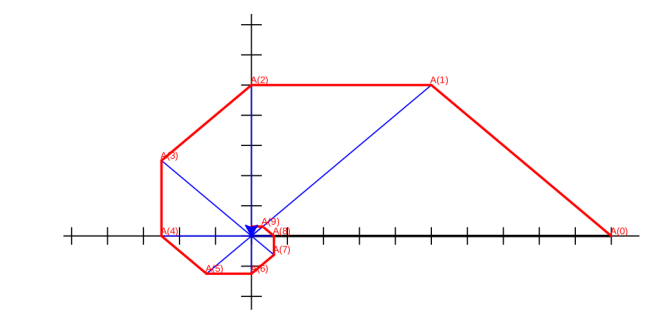
\includegraphics[scale=0.2]{images/capacite8.png}
\end{center}



Pour tout entier $n\geqslant 0$, on note $a_{n}$ la longueur $OA_{n}$ et $b_{n}$ la longueur $A_{n}A_{n+1}$.


\begin{itemize}
	\pause \item Pour tout entier $n\geqslant 0$, le triangle $OA_{n}A_{n+1}$ est rectangle isocèle en $A_{n+1}$ donc $OA_{n+1}=AA_{n} \times \cos \left(\frac{\pi}{4}\right)$ donc $a_{n+1}=\frac{\sqrt{2}}{2}a_{n}$. De plus $OA_{n}A_{n+1}$ isocèle en $A_{n+1}$  donc $A_{n}A_{n+1}=OA_{n+1}$, donc $b_{n}=a_{n+1}$ et donc $b_{n}=\frac{\sqrt{2}}{2}b_{n-1}$ pour tout entier $n \geqslant 1$.
	
\pause \item Les suites $(a_{n})$ et $(b_{n})$ sont donc identiques et ce sont des suites géométriques de premiers termes $a_{0}=1$ et $b_{0}=a_{1}=\frac{\sqrt{2}}{2}$.

\end{itemize}


\end{frame}




\begin{frame}
\frametitle{Capacité 8 Question 2}


\begin{center}
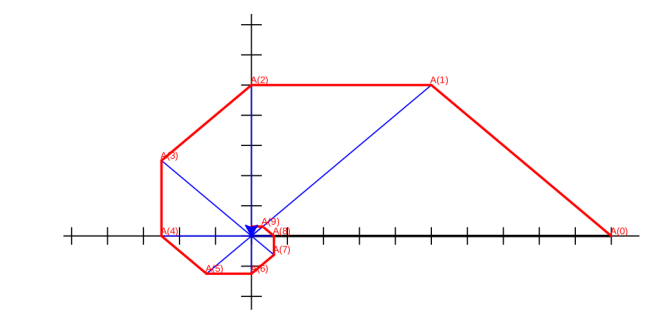
\includegraphics[scale=0.2]{images/capacite8.png}
\end{center}



Pour tout entier $n\geqslant 0$, on note $a_{n}$ la longueur $OA_{n}$ et $b_{n}$ la longueur $A_{n}A_{n+1}$.


\begin{itemize}
	\pause \item  D'après une propriété du cours sur les suites géométriques, pour tout entier $n \geqslant 0$, on a :  
\begin{align*}
a_{n} &=\left(\frac{\sqrt{2}}{2}\right)^{n}a_{0}=\left(\frac{\sqrt{2}}{2}\right)^{n}\\
b_{n} &=\left(\frac{\sqrt{2}}{2}\right)^{n}b_{0}=\left(\frac{\sqrt{2}}{2}\right)^{n+1}
\end{align*}
	

\end{itemize}


\end{frame}




\begin{frame}
\frametitle{Capacité 8 Question 3}


\begin{center}
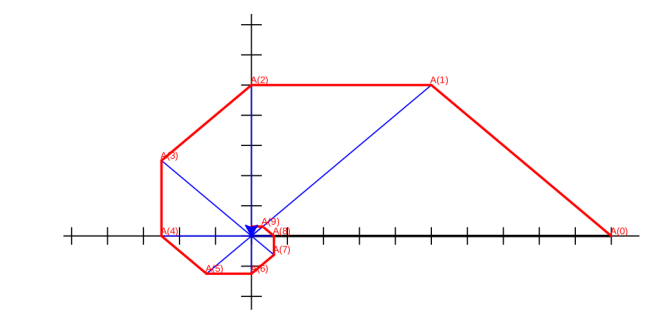
\includegraphics[scale=0.2]{images/capacite8.png}
\end{center}



Pour tout entier $n\geqslant 0$, on note $a_{n}$ la longueur $OA_{n}$ et $b_{n}$ la longueur $A_{n}A_{n+1}$.


\begin{itemize}

	
\pause \item Avec la calculatrice, on peut conjecturer que les suites $(a_{n})$  et $(b_{n})$ tendent vers $0$. On verra en terminale que cette propriété est liée à la valeur absolue de la raison qui est strictement inférieure à $1$. 

\end{itemize}


\end{frame}


\begin{frame}
\frametitle{Capacité 8 Question 4}


\begin{center}
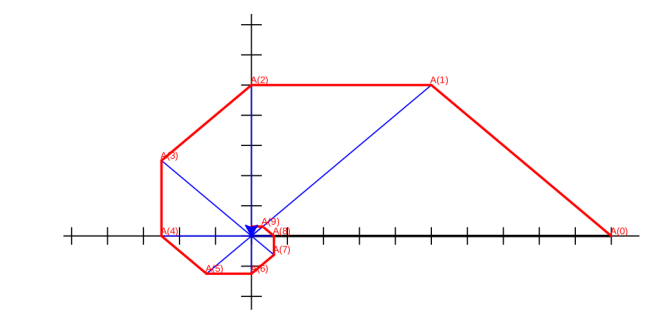
\includegraphics[scale=0.15]{images/capacite8.png}
\end{center}



On considère la  spirale constituée des segments $[A_{0}A_{1}]$, $[A_{1}A_{2}]$, \ldots, $[A_{n-1}A_{n}]$. 

\begin{itemize}
	\pause \item La longueur de la spirale est égale  la somme des $n$ premiers termes termes de la suite $(b_{n})$ : $b_{0}+b_{1}+\ldots + b_{n}$.
	
	
\pause \item D'après une propriété du cours sur les suites géométriques : 
\begin{align*}
b_{0}+b_{1}+\ldots+b_{n} &=b_{0} \times \frac{1- \left(\frac{\sqrt{2}}{2}\right)^{n}}{1 - \frac{\sqrt{2}}{2}} 
\end{align*}
En reprenant le raisonnement de la question précédente, on peut conjecturer que $b_{0}+b_{1}+\ldots+b_{n}$ tend vers  
$\frac{\sqrt{2}}{2} \times \frac{1}{1 - \frac{\sqrt{2}}{2}}$ lorsque $n$ tend vers $+\infty$.
\end{itemize}


\end{frame}


\begin{frame}
\frametitle{Capacité 9}
\label{capacite9}

\begin{itemize}
\item Un exemple de suite de limite $734$  :  $(u_{n})$ définie pour tout entier $n \geqslant 0$ par $u_{n}=734+0,5^{n}$ ;
\item Un exemple de suite de limite $+\infty$ : $(u_{n})$ définie pour tout entier $n \geqslant 0$ par $u_{n}=n$ ;
\item Un exemple de suite de limite $-\infty$ : $(u_{n})$ définie pour tout entier $n \geqslant 0$ par $u_{n}=-n$ ;
\item Un exemple de suite bornée sans limite : $(u_{n})$ définie pour tout entier $n \geqslant 0$ par $u_{n}=\cos(n)$ ;
\item Un exemple de suite non bornée sans limite : $(u_{n})$ définie pour tout entier $n \geqslant 0$ par $u_{n}=n\cos(n)$.
\end{itemize}

\end{frame}



\end{document}